\chapter{Results}
This chapter reports the empirical performance of the three Linux translation implementations relative to a native Dual-Stack baseline in the three environments described in Chapter 4. The evaluation isolates the translation overhead of a CLAT-based path along two metrics: TCP throughput and ICMP round-trip time (RTT). Within each environment, comparisons are made relative to the IPv6 baseline to control for differences in virtualization and CPU topology across environments. Sections 5.1 and 5.2 present the throughput and RTT results, respectively. The last section of this chapter, section 5.3 discusses the findings.

\section{Throughput}
All throughput plots show time in seconds on the x-axis and throughput in Gbit/s on the y-axis and depict iperf3 time series over the configured measurement window\footnote{The scripts used for generating all plots and analyzing the measurement data are available at: \url{https://github.com/thisIsDanielJin/bachelorthesis_scripts.git}}. The AWS environment is considered first to set the stage for later changes in timing configuration and platform.
The initial AWS measurement, which can be seen in Figure \ref{fig:AWS_tcp_sameScale_kvm-clock_linear}, run with the default kvm-clock shows a divergence in behavior between the user-space translators and Jool. Tayga and Tundra remain stable across repetitions, whereas both the native IPv6 baseline and Jool show large variability without a consistent trend. Since configuration, topology, and traffic generation were held constant, this pattern indicates platform caused timing artifacts rather than datapath specific instability. The clocksource was therefore assumed to be the primary source of variance, and following runs replaced kvm-clock with hpet to test this hypothesis.

\begin{figure}[H]
    \centering
    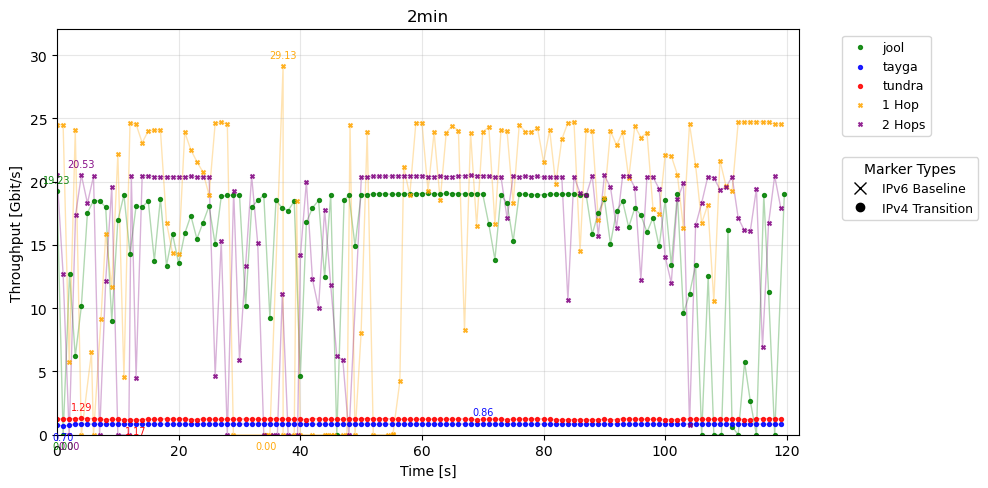
\includegraphics[width=1\textwidth]{resources/finalPlots/combinedplots/AWS_tcp_sameScale_kvm-clock_2min_linear.png}
    \caption{AWS throughput, KVM-clock, linear scale}
    \label{fig:AWS_tcp_sameScale_kvm-clock_linear}

\end{figure}

Switching to hpet (Figure \ref{fig:AWS_tcp_sameScale_hpet_log}) reduces anomalies but does not fully eliminate irregular throughput steps for the IPv6 baseline. Because the native baseline clusters near the top of the axis while the CLAT implementations cluster near the bottom, a dual-y-axis variant (Figure \ref{fig:AWS_tcp_dualAxis_hpet_log}) improves readability by separating the dynamic ranges without altering the underlying samples. The left y-axis scales the IPv6 baseline and the right y-axis scales the CLAT datapaths. Even here, the baseline still shows a step-like pattern, which is consistent with the remaining jitter. These results support the decision to move the same experimental topology to a bare-metal machine in order to reduce noise.


\begin{figure}[H]
    \centering
    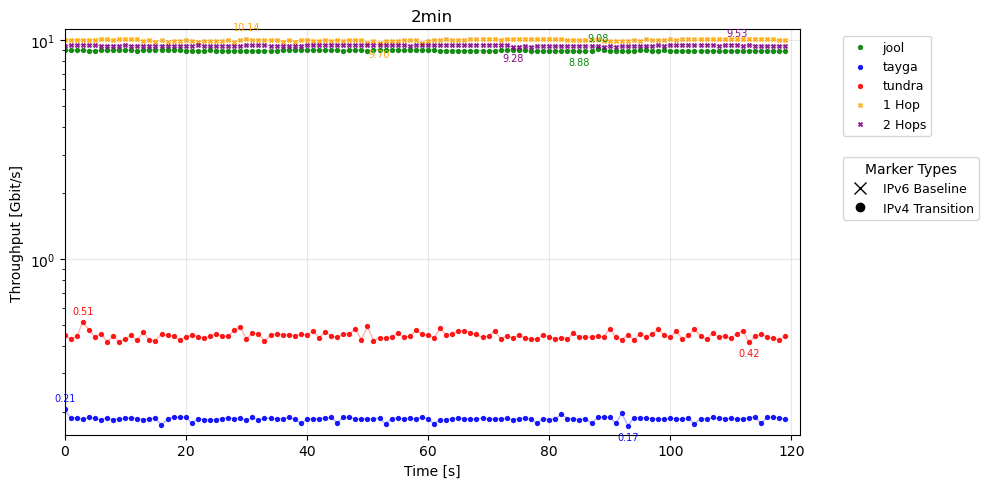
\includegraphics[width=1\textwidth]{resources/finalPlots/combinedplots/AWS_tcp_sameScale_hpet_2min_log.png}
    \caption{AWS throughput, hpet, log scale}
    \label{fig:AWS_tcp_sameScale_hpet_log}

\end{figure}


\begin{figure}[H]
    \centering
    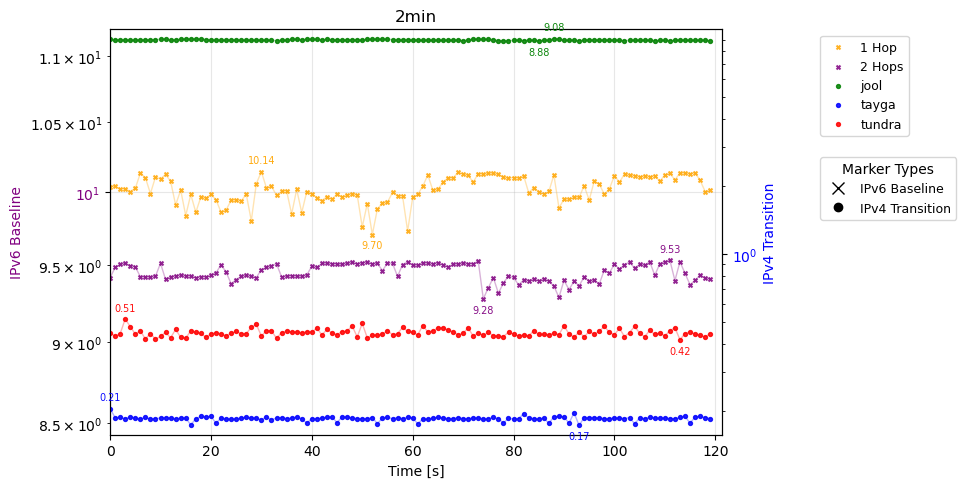
\includegraphics[width=1\textwidth]{resources/finalPlots/Jitterplots/AWS_tcp_dualAxis_hpet_2min_log.png}
    \caption{AWS Throughput, hpet, dual-y-axis, log scale}
    \label{fig:AWS_tcp_dualAxis_hpet_log}
\end{figure}



\paragraph{Bare-metal results}

On the bare-metal host (Figure \ref{fig:Local_tcp_sameScale_tsc_linear}), throughput stabilizes for both baseline and CLAT paths. The results show tight clustering across repetitions and a clear separation between one-hop and two-hop IPv6 baselines, consistent with the additional namespace traversal. Specifically, the one-hop baseline averages 42.039 Gbit/s and median of 42.215 Gbit/s, while the two-hop baseline averages 35.131 Gbit/s with median of 35.852 Gbit/s, which matches expectations for an extra hop. Within this environment, Jool consistently outperforms Tundra. Under TSC, Jool reaches a mean of about 33.81 Gbit/s versus 4.42 Gbit/s for Tundra. Under hpet, Jool's mean is about 6.64 Gbit/s versus 0.51 Gbit/s for Tundra. Tayga is not shown here due to the reasons summarized in Section 5.3. Because Tayga and Tundra are both stateless user-space translators with similar behavior, Tundra serves as a representative for this class in the bare-metal host setup, which is also in line with the AWS observations where Tayga and Tundra track closely.

\begin{figure}[H]
    \centering
    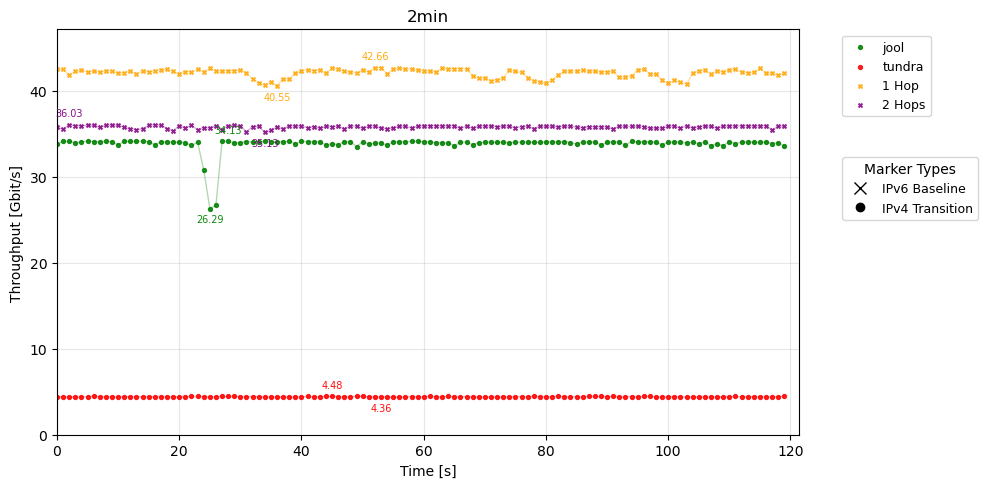
\includegraphics[width=1\textwidth]{resources/finalPlots/combinedplots/SingleLocal_tcp_sameScale_tsc_2min_linear.png}
    \caption{Bare-metal host, throughput, tsc, linear scale}
    \label{fig:Local_tcp_sameScale_tsc_linear}
\end{figure}

For consistency we also switched the clocksource to hpet in the bare-metal host environment (Figure \ref{fig:Local_tcp_sameScale_hpet_linear}).

\begin{figure}[H]
    \centering
    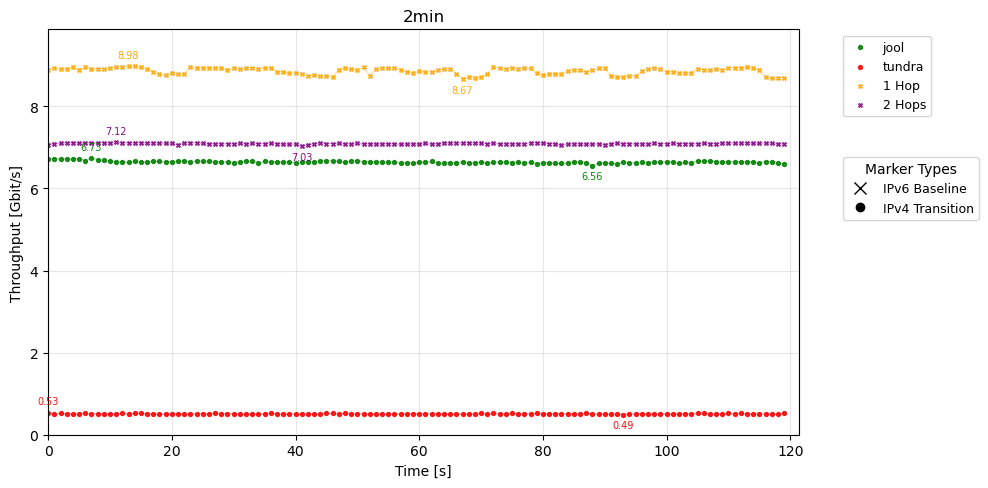
\includegraphics[width=1\textwidth]{resources/finalPlots/combinedplots/SingleLocal_tcp_sameScale_hpet_2min_linear.png}
    \caption{Bare-metal host, throughput, hpet, linear scale}
    \label{fig:Local_tcp_sameScale_hpet_linear}
\end{figure}

Figure \ref{fig:Local_tcp_dualAxis_hpet_linear} illustrates, in contrast to the earlier AWS dual-y-axis plot, a significantly more stable IPv6 baseline and a clear distinction between the two CLAT implementations.

\begin{figure}[H]
    \centering
    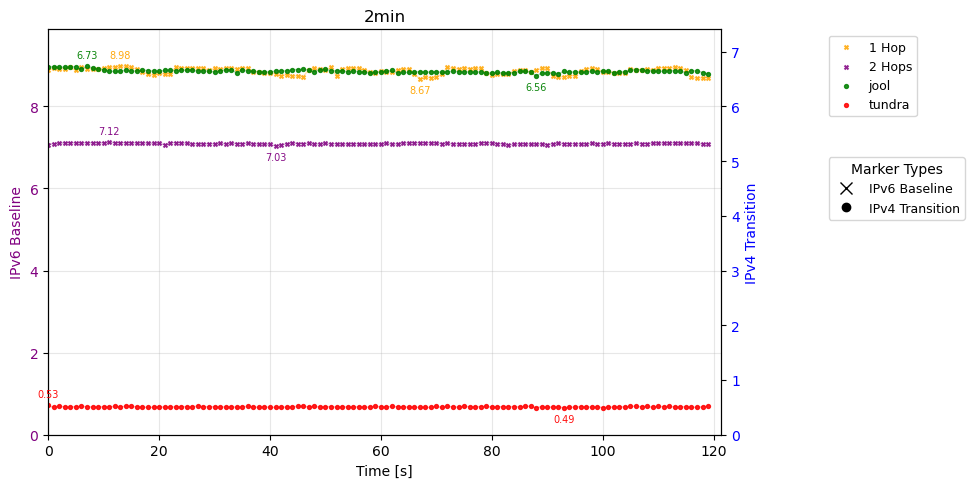
\includegraphics[width=1\textwidth]{resources/finalPlots/Jitterplots/LocalSingle_tcp_dualAxis_hpet_2min_linear.png}
    \caption{Bare-metal host, throughput, hpet, dual-y-axis, linear scale}
    \label{fig:Local_tcp_dualAxis_hpet_linear}
\end{figure}



Moving on the bare-metal network setup (Figure \ref{fig:Dual_tcp_sameScale_hpet_log}), it introduces a physical 1 Gbit/s Ethernet link that caps the achievable throughput for all datapaths. In this environment, the absolute advantage of the kernel-space datapath on loopback is compressed by the link bottleneck, and both Jool and Tundra approach the capacity limit. Jool peaks at 0.66 Gbit/s while Tundra approaches 0.57 Gbit/s and the IPv6 baselines are bounded by 1 Gbit/s as expected under both TSC and hpet. The slight upward trends over time are caused by TCP congestion control behavior\cite{rfc5681} but does not affect the ordering of the results. The key observation is that when the bottleneck is the external link rather than the host datapath, the differences between CLAT implementations become small relative to the link capacity, and the gap to the dual-stack baseline largely disappears.


\begin{figure}[H]
    \centering
    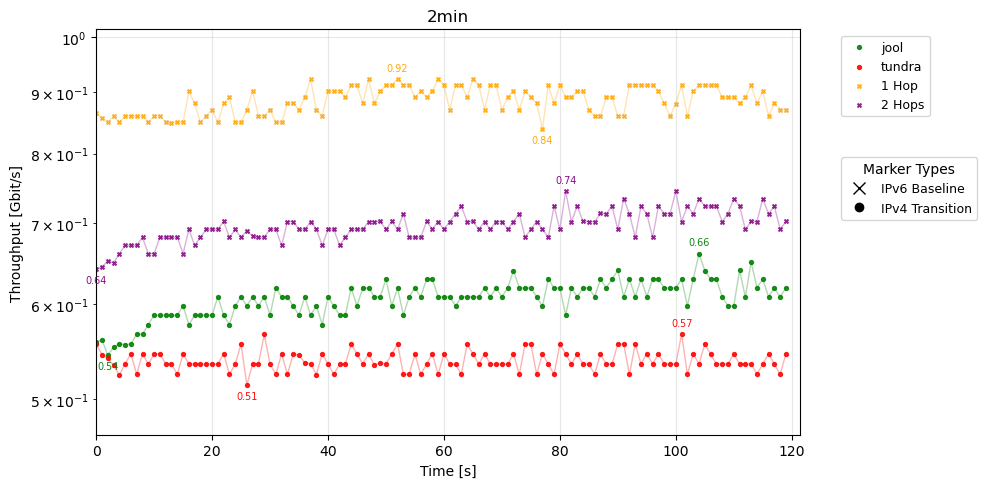
\includegraphics[width=1\textwidth]{resources/finalPlots/combinedplots/DoubleLocal_tcp_sameScale_hpet_2min_log.png}
    \caption{Bare-metal network, throughput, hpet, log scale}
    \label{fig:Dual_tcp_sameScale_hpet_log}
\end{figure}

The tsc results in Figure \ref{fig:Dual_tcp_sameScale_tsc_log} exhibit an artifact in which all plots oscillate between 0.92 and 0.93 Gbit/s. As discussed in Chapter 4, this behavior arises from the way TSC operates. Although all values are constrained by the 1 Gbit/s link, the low-resolution clock source of TSC causes the measurements to cluster tightly around the link limit. The observed oscillation is therefore a measurement artifact rather than an inherent property of the datapaths. This effect does not appear when using hpet, whose lower resolution and higher jitter smooth out the measurements.

\begin{figure}[H]
    \centering
    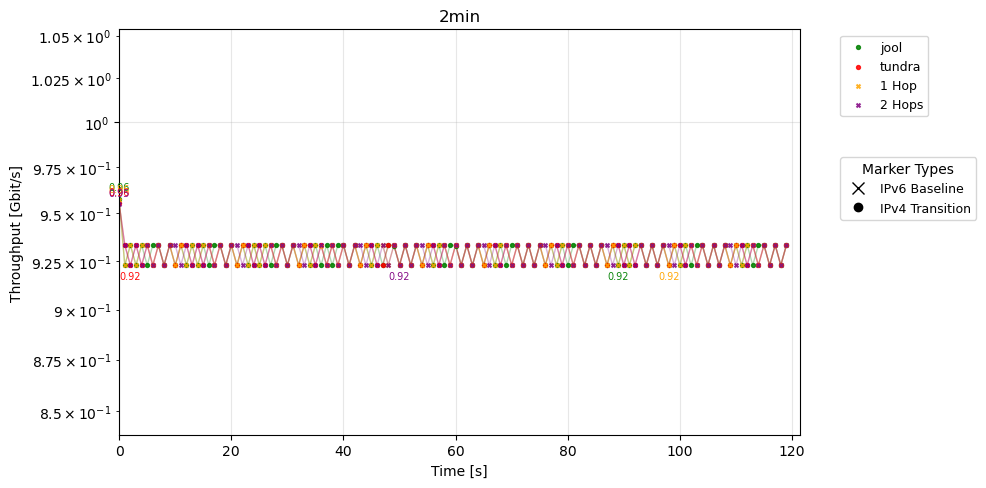
\includegraphics[width=1\textwidth]{resources/finalPlots/combinedplots/DoubleLocal_tcp_sameScale_tsc_2min_log.png}
    \caption{Bare-metal network, throughput, tsc, log scale}
    \label{fig:Dual_tcp_sameScale_tsc_log}
\end{figure}

Looking at the dual-y-axis plot in Figure \ref{fig:Double_tcp_dualAxis_hpet_log} for this scenario, the IPv6 baseline shows a stable throughput compared to the AWS environment.
\begin{figure}[H]
    \centering
    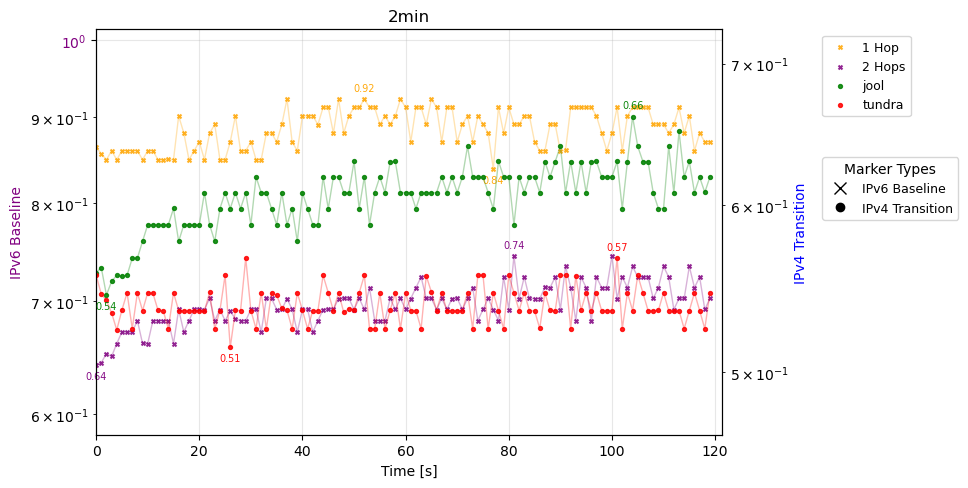
\includegraphics[width=1\textwidth]{resources/finalPlots/Jitterplots/LocalDouble_tcp_dualAxis_hpet_2min_log.png}
    \caption{Bare-metal network, throughput, hpet, dual-y-axis, log scale}
    \label{fig:Double_tcp_dualAxis_hpet_log}
\end{figure}

Across environments, two effects stand out. First, the translation overhead of CLAT relative to a native IPv6 baseline is strongly environment-dependent. On loopback, Jool’s kernel datapath yields a substantial advantage over user-space due to fewer context switches and reduced packet copy overhead, while on a 1 Gbit/s physical link the advantage compresses toward the link limit. Second, clocksource selection has a measurable impact on time series smoothness and on the dispersion of repeated measurements, especially under virtualization. The bare-metal results show that platform-induced jitter can dominate differences in the cloud.

\section{RTT}
The RTT results mirror the throughput analysis in showing that the translation cost is small and that kernel-space translation retains a consistent advantage over user-space, while environment and topology shape absolute values. In the AWS environment under hpet (Figure \ref{fig:AWS_icmp_sameScale_hpet_log}), a clear gap separates the IPv6 baselines from the CLAT datapaths, consistent with the expectation that translation introduces additional per-packet processing. The one hop IPv6 baseline has a median at 0.042 ms and the two hop baseline around 0.053 ms. Among translators, Jool achieves a mean of 0.064 ms, while Tayga and Tundra lie around 0.091 ms and 0.099 ms, respectively. The relative ordering is therefore consistent with the throughput results.


\begin{figure}[H]
    \centering
    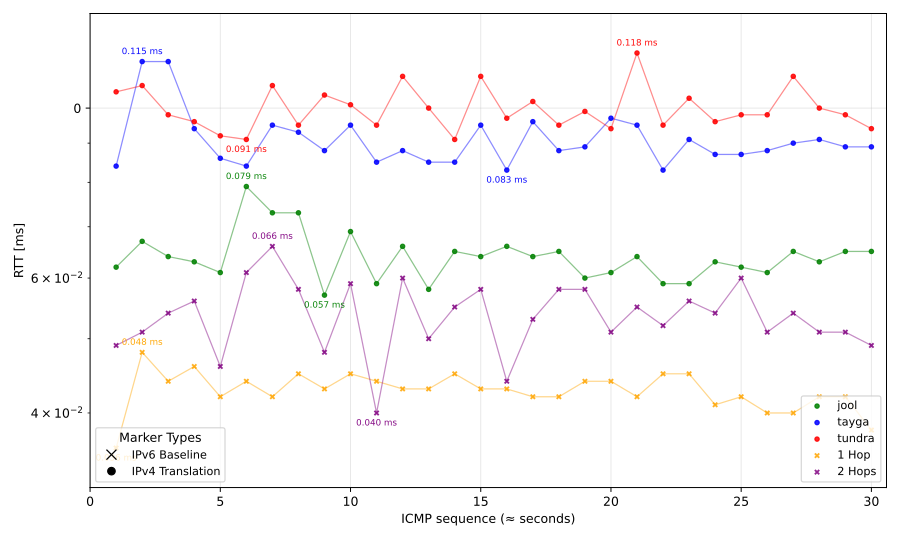
\includegraphics[width=1\textwidth]{resources/plots/CombinedPlot/RTT/AWS_ping_rtt_Ping_30s_log.png}
    \caption{AWS RTT, hpet, log scale}
    \label{fig:AWS_icmp_sameScale_hpet_log}

\end{figure}

On the bare-metal host (Figure \ref{fig:Local_icmp_sameScale_hpet_linear}), RTTs increase across all datapaths relative to AWS, which is explained by the host’s lower CPU performance. The ordering remains unchanged: Jool again exhibits the lowest CLAT latency with a mean of 0.189 ms, while Tundra’s mean is around 0.24 ms. The spread within each series is narrower than in AWS, consistent with the reduced timing jitter observed for throughput.

\begin{figure}[H]
    \centering
    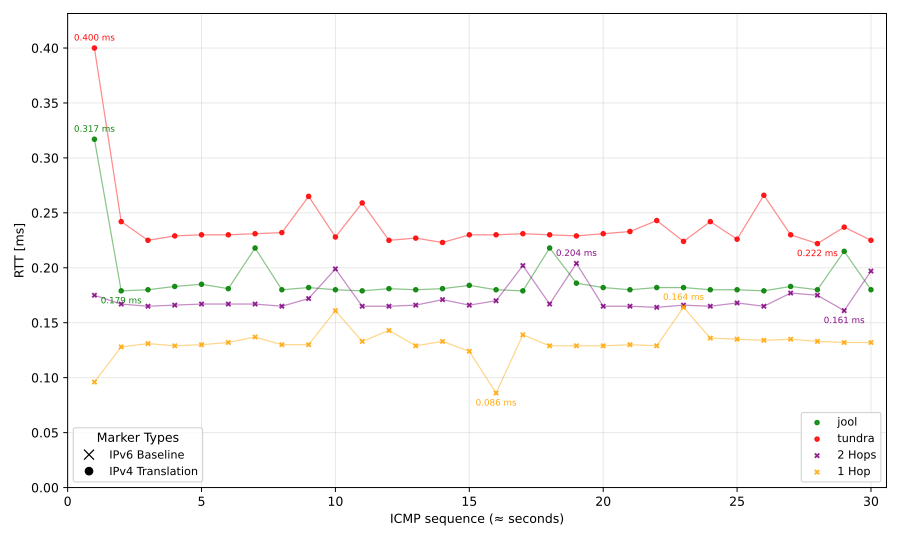
\includegraphics[width=1\textwidth]{resources/plots/CombinedPlot/RTT/Single_ping_rtt_Ping_30s_linear.png}
    \caption{Bare-metal host, RTT, hpet, linear scale}
    \label{fig:Local_icmp_sameScale_hpet_linear}
\end{figure}

The bare-metal network environment (Figure \ref{fig:Dual_icmp_sameScale_hpet_log}) produces the highest RTTs due to the additional physical hop traversing the Ethernet link. Variability increases across all datapaths, reflecting the added queueing opportunities along the path. Despite the shift in absolute values, the relative ordering persists, with Jool maintaining a modest latency advantage over user-space translation. The gap to the IPv6 baselines remains small in absolute terms, which supports the thesis that CLAT overhead is limited in practice.


\begin{figure}[H]
    \centering
    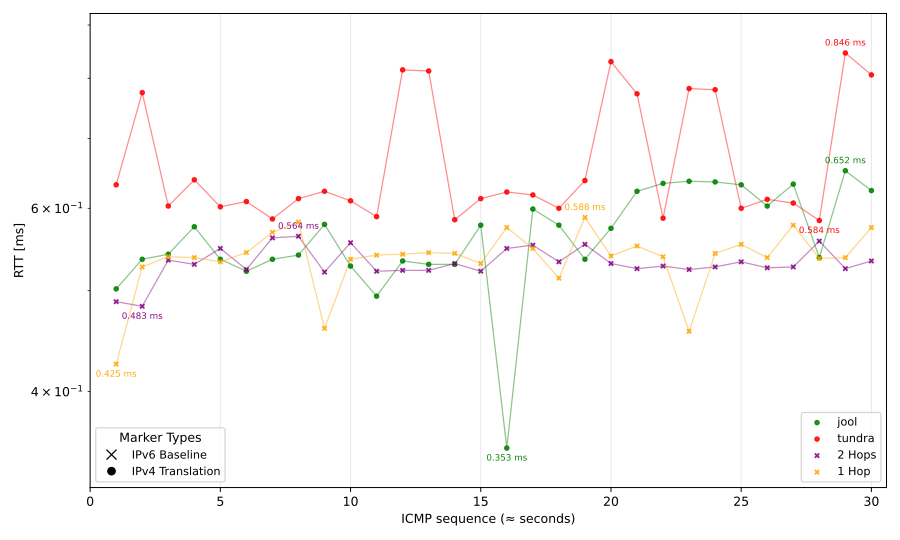
\includegraphics[width=1\textwidth]{resources/plots/CombinedPlot/RTT/Double_ping_rtt_Ping_30s_log.png}
    \caption{Bare-metal network, RTT, hpet, log scale}
    \label{fig:Dual_icmp_sameScale_hpet_log}
\end{figure}

The following tables~\ref{tab:rtt_comparison}, \ref{tab:throughput_comparison_aws}, \ref{tab:throughput_comparison_localsingle}, and~\ref{tab:throughput_comparison_localdouble} summarize the key statistics across all measurement scenarios.

\begin{table}[htbp]
\centering
\caption{RTT Performance Comparison Across Translation Tools and Scenarios}
\label{tab:rtt_comparison}
\footnotesize
\begin{tabular}{|l|c|l|r|r|r|r|r|r|}
\hline
\textbf{Scenario} & \textbf{Type} & \textbf{Tool} & \textbf{Min} & \textbf{Avg} & \textbf{Median} & \textbf{Max} & \textbf{Std Dev} & \textbf{P95}  \\
 & & & \textbf{(ms)} & \textbf{(ms)} & \textbf{(ms)} & \textbf{(ms)} & \textbf{(ms)} & \textbf{(ms)}  \\
\hline
AWS & IPv4 & Jool & 0.057 & 0.064 & 0.064 & 0.079 & 0.005 & 0.073   \\
AWS & IPv4 & Tayga & 0.083 & 0.091 & 0.089 & 0.115 & 0.008 & 0.107   \\
AWS & IPv4 & Tundra & 0.091 & 0.099 & 0.098 & 0.118 & 0.006 & 0.110   \\
AWS & Baseline & Tundra & 0.036 & 0.042 & 0.043 & 0.048 & 0.002 & 0.046   \\
AWS & Baseline & Jool & 0.040 & 0.053 & 0.054 & 0.066 & 0.005 & 0.061   \\
AWS & Baseline & Tayga & 0.033 & 0.042 & 0.043 & 0.049 & 0.004 & 0.048   \\
\hline
Bare-metal host & IPv4 & Jool & 0.179 & 0.189 & 0.181 & 0.317 & 0.026 & 0.218   \\
Bare-metal host & IPv4 & Tundra & 0.222 & 0.239 & 0.230 & 0.400 & 0.032 & 0.266   \\
Bare-metal host & Baseline & Jool & 0.161 & 0.171 & 0.167 & 0.204 & 0.012 & 0.201   \\
Bare-metal host & Baseline & Tundra & 0.086 & 0.131 & 0.132 & 0.164 & 0.014 & 0.153   \\
Bare-metal host & Baseline & Tayga & 0.122 & 0.134 & 0.127 & 0.251 & 0.024 & 0.167   \\
\hline
Bare-metal network & IPv4 & Jool & 0.353 & 0.563 & 0.558 & 0.652 & 0.060 & 0.637   \\
Bare-metal network & IPv4 & Tundra & 0.584 & 0.666 & 0.615 & 0.846 & 0.091 & 0.823   \\
Bare-metal network & Baseline & Jool & 0.483 & 0.532 & 0.529 & 0.564 & 0.018 & 0.560   \\
Bare-metal network & Baseline & Tundra & 0.425 & 0.537 & 0.540 & 0.588 & 0.035 & 0.580   \\
Bare-metal network & Baseline & Tayga & 0.403 & 0.539 & 0.540 & 0.577 & 0.037 & 0.575   \\
\hline
\end{tabular}
\end{table}

\begin{table}[htbp]
\centering
\caption{AWS Cloud Environment Throughput Performance Comparison}
\label{tab:throughput_comparison_aws}
\footnotesize
\begin{tabular}{|l|l|l|l|r|r|r|r|r|r|}
\hline
\textbf{Clock-} & \textbf{Time} & \textbf{Type} & \textbf{Tool} & \textbf{Min} & \textbf{Avg} & \textbf{Median} & \textbf{Max} & \textbf{Std Dev} & \textbf{P95} \\
\textbf{source} & & & & \textbf{(Gbps)} & \textbf{(Gbps)} & \textbf{(Gbps)} & \textbf{(Gbps)} & \textbf{(Gbps)} & \textbf{(Gbps)} \\
\hline
hpet & 30s & IPv4 & Tayga & 0.176 & 0.187 & 0.186 & 0.209 & 0.005 & 0.193 \\
hpet & 30s & IPv4 & Tundra & 0.398 & 0.432 & 0.433 & 0.454 & 0.012 & 0.450 \\
hpet & 30s & IPv4 & Jool & 8.929 & 9.021 & 9.014 & 9.094 & 0.039 & 9.090 \\
hpet & 30s & Baseline & Tayga & 9.921 & 10.062 & 10.083 & 10.160 & 0.069 & 10.140 \\
hpet & 30s & Baseline & Jool & 9.362 & 9.418 & 9.398 & 9.516 & 0.050 & 9.511 \\
hpet & 30s & Baseline & Tundra & 9.908 & 9.996 & 9.982 & 10.119 & 0.054 & 10.111 \\
hpet & 2min & IPv4 & Jool & 8.884 & 8.964 & 8.958 & 9.082 & 0.043 & 9.037 \\
hpet & 2min & IPv4 & Tayga & 0.173 & 0.186 & 0.187 & 0.205 & 0.004 & 0.190 \\
hpet & 2min & IPv4 & Tundra & 0.416 & 0.447 & 0.445 & 0.515 & 0.016 & 0.477 \\
hpet & 2min & Baseline & Tundra & 9.705 & 10.016 & 10.014 & 10.142 & 0.093 & 10.130 \\
hpet & 2min & Baseline & Tayga & 9.714 & 10.079 & 10.111 & 10.188 & 0.094 & 10.180 \\
hpet & 2min & Baseline & Jool & 9.276 & 9.451 & 9.445 & 9.530 & 0.056 & 9.519 \\
\hline
kvm & 30s & IPv4 & Tayga & 0.732 & 0.834 & 0.842 & 0.854 & 0.027 & 0.851 \\
kvm & 30s & IPv4 & Tundra & 1.205 & 1.236 & 1.235 & 1.286 & 0.021 & 1.270 \\
kvm & 30s & IPv4 & Jool & 0.001 & 15.995 & 17.840 & 18.967 & 4.426 & 18.929 \\
kvm & 30s & Baseline & Tayga & 0.000 & 14.808 & 19.622 & 24.638 & 9.113 & 24.214 \\
kvm & 30s & Baseline & Jool & 11.579 & 19.922 & 20.824 & 20.955 & 2.134 & 20.903 \\
kvm & 30s & Baseline & Tundra & 14.209 & 23.299 & 24.482 & 24.732 & 2.653 & 24.688 \\
kvm & 2min & IPv4 & Jool & 0.000 & 15.488 & 18.075 & 19.234 & 5.507 & 19.047 \\
kvm & 2min & IPv4 & Tayga & 0.703 & 0.838 & 0.841 & 0.861 & 0.019 & 0.854 \\
kvm & 2min & IPv4 & Tundra & 1.168 & 1.227 & 1.228 & 1.288 & 0.028 & 1.271 \\
kvm & 2min & Baseline & Tundra & 0.000 & 17.034 & 21.558 & 29.127 & 9.261 & 24.690 \\
kvm & 2min & Baseline & Tayga & 0.000 & 17.865 & 23.146 & 24.881 & 8.718 & 24.835 \\
kvm & 2min & Baseline & Jool & 0.000 & 16.228 & 20.346 & 20.525 & 6.637 & 20.474 \\
\hline
\end{tabular}
\end{table}


\begin{table}[htbp]
\centering
\caption{Bare-metal host Throughput Performance Comparison}
\label{tab:throughput_comparison_localsingle}
\footnotesize
\begin{tabular}{|l|l|l|l|r|r|r|r|r|r|}
\hline
\textbf{Clock-} & \textbf{Time} & \textbf{Type} & \textbf{Tool} & \textbf{Min} & \textbf{Avg} & \textbf{Median} & \textbf{Max} & \textbf{Std Dev} & \textbf{P95} \\
\textbf{source} & & & & \textbf{(Gbps)} & \textbf{(Gbps)} & \textbf{(Gbps)} & \textbf{(Gbps)} & \textbf{(Gbps)} & \textbf{(Gbps)} \\
\hline
hpet & 30s & IPv4 & Tundra & 0.495 & 0.518 & 0.520 & 0.537 & 0.008 & 0.527 \\
hpet & 30s & IPv4 & Jool & 6.677 & 6.746 & 6.757 & 6.786 & 0.028 & 6.771 \\
hpet & 30s & Baseline & Tayga & 8.678 & 8.868 & 8.937 & 8.968 & 0.109 & 8.961 \\
hpet & 30s & Baseline & Jool & 6.984 & 7.090 & 7.105 & 7.114 & 0.033 & 7.113 \\
hpet & 30s & Baseline & Tundra & 8.706 & 8.900 & 8.905 & 9.038 & 0.100 & 9.019 \\
hpet & 2min & IPv4 & Jool & 6.557 & 6.644 & 6.642 & 6.735 & 0.028 & 6.714 \\
hpet & 2min & IPv4 & Tundra & 0.493 & 0.510 & 0.510 & 0.535 & 0.007 & 0.521 \\
hpet & 2min & Baseline & Tayga & 8.674 & 8.852 & 8.876 & 8.942 & 0.070 & 8.927 \\
hpet & 2min & Baseline & Tundra & 8.670 & 8.860 & 8.891 & 8.977 & 0.080 & 8.948 \\
hpet & 2min & Baseline & Jool & 7.033 & 7.092 & 7.092 & 7.121 & 0.015 & 7.112 \\
\hline
tsc & 30s & IPv4 & Tundra & 4.394 & 4.435 & 4.435 & 4.477 & 0.020 & 4.464 \\
tsc & 30s & IPv4 & Jool & 33.255 & 33.873 & 33.929 & 34.084 & 0.181 & 34.060 \\
tsc & 30s & Baseline & Tayga & 41.221 & 42.328 & 42.521 & 42.888 & 0.550 & 42.885 \\
tsc & 30s & Baseline & Jool & 35.586 & 35.879 & 35.932 & 36.082 & 0.139 & 36.034 \\
tsc & 30s & Baseline & Tundra & 41.615 & 42.307 & 42.340 & 42.977 & 0.294 & 42.685 \\
tsc & 2min & IPv4 & Jool & 26.289 & 33.813 & 34.015 & 34.131 & 1.008 & 34.105 \\
tsc & 2min & IPv4 & Tundra & 4.362 & 4.417 & 4.415 & 4.478 & 0.025 & 4.455 \\
tsc & 2min & Baseline & Tayga & 40.713 & 42.063 & 42.229 & 42.839 & 0.585 & 42.763 \\
tsc & 2min & Baseline & Tundra & 40.553 & 42.039 & 42.215 & 42.658 & 0.496 & 42.572 \\
tsc & 2min & Baseline & Jool & 35.131 & 35.778 & 35.842 & 36.032 & 0.167 & 35.967 \\
\hline
\end{tabular}
\end{table}

\begin{table}[htbp]
\centering
\caption{Bare-metal network Throughput Performance Comparison}
\label{tab:throughput_comparison_localdouble}
\footnotesize
\begin{tabular}{|l|l|l|l|r|r|r|r|r|r|}
\hline
\textbf{Clock-} & \textbf{Time} & \textbf{Type} & \textbf{Tool} & \textbf{Min} & \textbf{Avg} & \textbf{Median} & \textbf{Max} & \textbf{Std Dev} & \textbf{P95} \\
\textbf{source} & & & & \textbf{(Gbps)} & \textbf{(Gbps)} & \textbf{(Gbps)} & \textbf{(Gbps)} & \textbf{(Gbps)} & \textbf{(Gbps)} \\
\hline
hpet & 30s & IPv4 & Tundra & 0.524 & 0.541 & 0.538 & 0.566 & 0.010 & 0.559 \\
hpet & 30s & IPv4 & Jool & 0.540 & 0.584 & 0.587 & 0.608 & 0.019 & 0.608 \\
hpet & 30s & Baseline & Tayga & 0.848 & 0.859 & 0.860 & 0.891 & 0.009 & 0.876 \\
hpet & 30s & Baseline & Jool & 0.631 & 0.672 & 0.676 & 0.703 & 0.019 & 0.692 \\
hpet & 30s & Baseline & Tundra & 0.837 & 0.856 & 0.849 & 0.891 & 0.012 & 0.876 \\
hpet & 2min & IPv4 & Jool & 0.544 & 0.606 & 0.608 & 0.661 & 0.021 & 0.630 \\
hpet & 2min & IPv4 & Tundra & 0.514 & 0.538 & 0.535 & 0.566 & 0.010 & 0.556 \\
hpet & 2min & Baseline & Tayga & 0.849 & 0.883 & 0.881 & 0.923 & 0.024 & 0.923 \\
hpet & 2min & Baseline & Tundra & 0.839 & 0.885 & 0.891 & 0.923 & 0.023 & 0.912 \\
hpet & 2min & Baseline & Jool & 0.641 & 0.696 & 0.692 & 0.745 & 0.020 & 0.724 \\
\hline
tsc & 30s & IPv4 & Tundra & 0.923 & 0.929 & 0.933 & 0.950 & 0.006 & 0.933 \\
tsc & 30s & IPv4 & Jool & 0.923 & 0.929 & 0.933 & 0.954 & 0.007 & 0.933 \\
tsc & 30s & Baseline & Tayga & 0.923 & 0.929 & 0.933 & 0.959 & 0.008 & 0.933 \\
tsc & 30s & Baseline & Jool & 0.923 & 0.929 & 0.933 & 0.949 & 0.006 & 0.933 \\
tsc & 30s & Baseline & Tundra & 0.923 & 0.929 & 0.933 & 0.959 & 0.008 & 0.933 \\
tsc & 2min & IPv4 & Jool & 0.923 & 0.929 & 0.933 & 0.958 & 0.006 & 0.933 \\
tsc & 2min & IPv4 & Tundra & 0.923 & 0.929 & 0.933 & 0.956 & 0.006 & 0.933 \\
tsc & 2min & Baseline & Tayga & 0.923 & 0.929 & 0.933 & 0.955 & 0.006 & 0.933 \\
tsc & 2min & Baseline & Tundra & 0.923 & 0.929 & 0.933 & 0.957 & 0.006 & 0.933 \\
tsc & 2min & Baseline & Jool & 0.923 & 0.929 & 0.933 & 0.955 & 0.006 & 0.933 \\
\hline
\end{tabular}
\end{table}

\section{Discussion}

Across the three environments, two technical factors consistently shaped the measurements more than the mere presence of translation: the location of the bottleneck (CPU/memory path versus network link) and the behavior of the system clocksource under the given platform. When the host datapath was the limiting resource, Jool achieved higher throughput and slightly lower RTT than the user space translators. This is consistent with expected mechanisms: fewer user/kernel context switches, fewer packet copies, and tighter cache locality in the kernel datapath. Contrarily, when a physical 1 Gbit/s link capped the rate, the differences among CLAT implementations compressed toward the link limit and the gap to the IPv6 baselines largely reflected the shared network bottleneck rather than translation.

Virtualization timing artifacts were clearly visible in the AWS environment. With kvm-clock, both the native IPv6 baseline and Jool exhibited large swings despite a constant topology and traffic profile, while Tayga and Tundra reported stable but lower throughputs. Switching to hpet reduced but did not eliminate irregular patterns in the IPv6 baseline time series. The divergence under kvm-clock and the residual artifacts under hpet indicate that timer behavior can overshadow datapath differences at high rates in virtualized settings. This observation motivated repeating the same topology on bare-metal machines, where platform-induced jitter was indeed reduced.

On bare metal, the role of the clocksource remained a first order effect. The tsc based runs produced tightly clustered, higher reported throughputs on loopback, while hpet yielded smoother traces with consistently lower throughputs. On the 1 Gbit/s ethernet link, tsc introduced a characteristic quantization around 0.92–0.93 Gbit/s for all datapaths, an artifact of timing resolution rather than a property of the translators, whereas hpet smoothed out the measurements at the cost of higher timing overhead. These patterns suggest that clock selection affects both the stability and the absolute levels of reported results, which in turn implies that comparisons should always be interpreted relative to a same-clock baseline.

Topology and hop count had a measurable, separate effect from translation. In the bare-metal host setup, the two-hop IPv6 baseline showed lower throughput than the one-hop IPv6 baseline. This baseline separation quantifies the cost of an extra namespace traversal and helps attribute what fraction of observed differences stems from topology rather than translation. It also supports reading the Jool versus user space gap on loopback as a combination of translation placement (kernel versus user space) and the additional hop required by the Jool setup.

Regarding the representation of user space translators, the plots for the bare-metal host throughput focus on Jool and Tundra. Two considerations motivated this choice. First, Tundra consistently outperformed Tayga in the AWS IPv4 translation tests, so including Tayga would not change the ordering and would add redundancy in the figures. Second, Tundra’s multi-threaded design makes it a reasonable user-space upper bound under the single-flow conditions used here. Using it as the representative user-space datapath simplifies comparisons while preserving the visibility of trends. Tayga remains included where it illuminates behavior (e.g., AWS throughput, baseline IPv6 throughput, and RTT tables) and its qualitative positioning relative to Tundra is consistent across environments.

The RTT results parallel the throughput findings. The kernel datapath retained a modest latency advantage over user space in all environments. Absolute RTTs were lowest on AWS, higher on the bare-metal host, and highest on the bare-metal network, consistent with CPU differences and the additional physical hop and queueing opportunities in the networked case. Variability was highest under virtualization and lowest on single-host bare metal, matching the throughput jitter patterns and reinforcing the role of timing sources and platform effects.
